
% Analizzando il requisito mi sono posto diverse domande: \\ \\
% \noindent{
%     \large\textit{Cosa significa dinamicamente?}
%     \normalsize{Il nostro obiettivo in questo caso è mostrare all'utente \textbf{contenuti diversi}
%     indipendentemente dal constesto e quindi dalla vista in cui si trova}\\ \\
%     \large\textit{Quale contesto?}
%     \normalsize{Con contesto dell'utente si intende lo stato attuale dell'applicazione,
%     quindi l'intero stack di navigazione se presente;
%     } \\ \\
% }

Prima di entrare nel merito delle soluzioni e problemi affrontati, elenco brevemente gli strumenti
base di iOS che mi sono stati utile nella progettazione e implementazione finale.

\section{Navigazione standard}

Un'applicazione iOS è un insieme di \textbf{UIViewController}\cite{viewcontroller} diversi che 
regolano ogni aspetto della lora vista;

% Qualsiasi applicazione ha infatti un rootViewController, ossia un ViewController di partenza

Ogni applicazione può avere degli \textbf{UINavigationController}\cite{navigationcontroller},
ossia dei contenitori di \textbf{UIViewController} che vengono
utilizzati per mantenere lo stack di navigazione e gestire la transizioni tra due UIViewController.

Nella figura~\ref{fig:1} si nota facilmente come un NavigationController gestisce un'array di ViewController e una sola 
navigation bar. \\
% In iOS sono infatti innate molte animazioni di navigazione che è utile sfruttare, piuttosto di creare 
% componenti custom poi difficili da rendere interattivi.\\

\begin{minipage}{\linewidth}
    \centering
    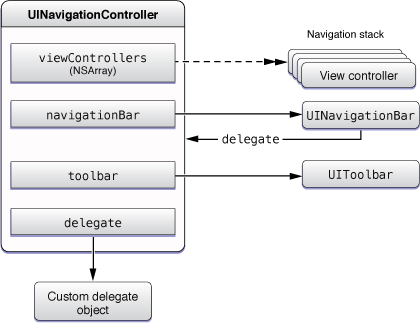
\includegraphics[width=5cm]{navigation}
    \captionof{figure}{Navigation controller scheme}
    \label{fig:1}
\end{minipage}

\subsection{Tipologie di navigazione}\label{sec:navigation}

Esistono tre tipologie base di navigazione:

\begin{enumerate}
    \item{\textbf{Push}: un UIViewController figlio di un NavigationController può rendere
    visibile un altro ViewController attraverso la funzione "pushViewController" di un Navigation controller\par
    \begin{minipage}{\linewidth}
        \centering
        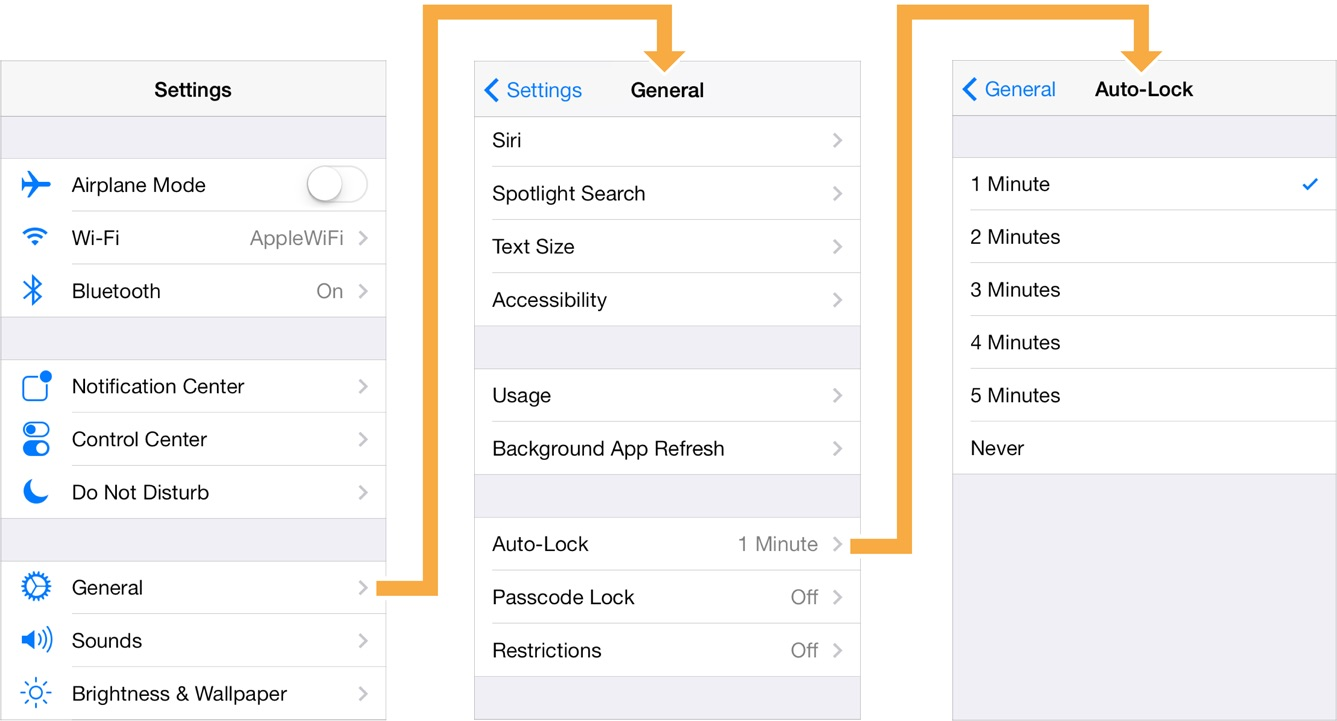
\includegraphics[width=10cm]{push}
        \captionof{figure}{Presantazione di un ViewController tramite push}
        \label{fig:2}
    \end{minipage}
    }
    \item{ \textbf{Modal}: un ViewController può presentare un altro ViewController senza necessariamente avere un 
        Navigation Controller, l'animazione standard è dal basso verso l'alto come in figura~\ref{fig:3}\par
        \begin{minipage}{\linewidth}
            \centering
            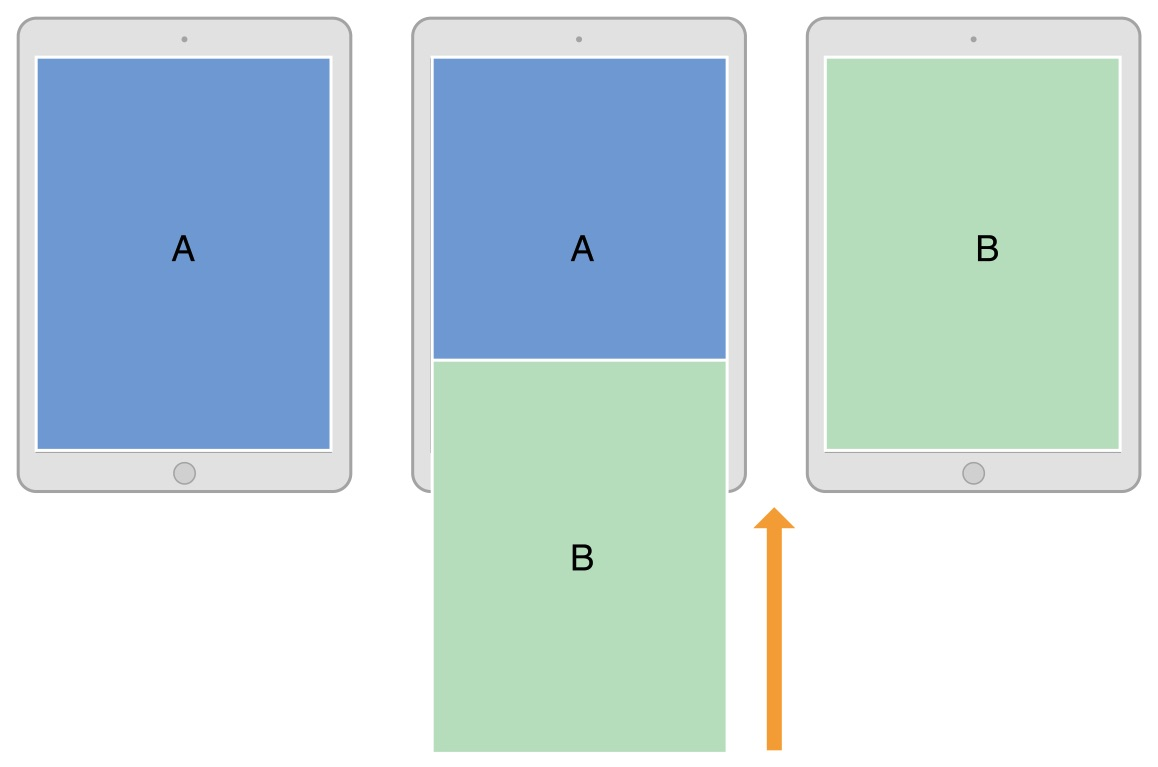
\includegraphics[width=10cm]{modal}
            \captionof{figure}{
                Presantazione di un ViewController tramite modal
            }
            \label{fig:3}
        \end{minipage}
    }
    \item{\textbf{Segue}: Una segue non è altro che un link tra due view controller attraverso un'interfaccia
        grafica. In base alla tipologia cambia il tipo di navigazione (Modal o Push)
    }
\end{enumerate}

% Avendo definito i principali metodi di navigatione tra ViewController torniamo al problema iniziale:
% \textit{Come possiamo rendere dinamica la navigazione?}

% A seguito di uno studio approfondito di varie tecniche di navigazione iOS ho scelto di utilizzare il
% \textbf{Coordinator Pattern}\cite{coordinatorpattern}.

% \section{Il Coordinator Pattern}

% Generalmente in iOS l'intera logica di un ViewController viene scritta nel ViewController stesso, creando spesso
% file di grosse dimensioni e disordine generale. Il Coordinator Pattern è nato proprio per rendere 
% le applicazioni più scalabili e leggere. 

% Ogni ViewController infatti delega tutte le decisioni al suo Coordinator che in base a determinate logiche deciderà
% i passi successivi.

% Ogni Coordinator può controllare un ViewController o più Coordinator, questo rende le viste
% indipendenti tra di loro e rende ogni ViewControler totalmente invisibile agli altri.\\

% \begin{minipage}{\linewidth}
%     \centering
%     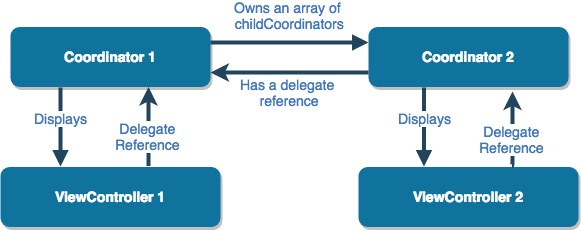
\includegraphics[width=10cm]{coordinator}
%     \captionof{figure}{
%         Il Coordinator Pattern
%     }
%     \label{fig:4}
% \end{minipage}\\ \\

% La resposibilità dei coordinator è infatti la navigazione, come un navigation controller gestisce i sui View Controller, un coordinator gestisce
% i suoi figli e questo rende ogni vista o flow di navigazione totalmente indipendente dal resto dell'applicazione.

% Per navigare tra i view controller vengono generalmente usate le tipologie di navigazione
% descritte nella sezione~\ref{sec:navigation}, tranne le segue, che essendo definete da vista grafica renderebbero
% la navigazine statica e fissata su determinati ViewController. \\

% Di seguito in figura~\ref{fig:5} presento uno schema dell'utilizzo di due coordinator
% per la gestione di una lista di prodotti e il carrello. \\

% \begin{minipage}{\linewidth}
%     \centering
%     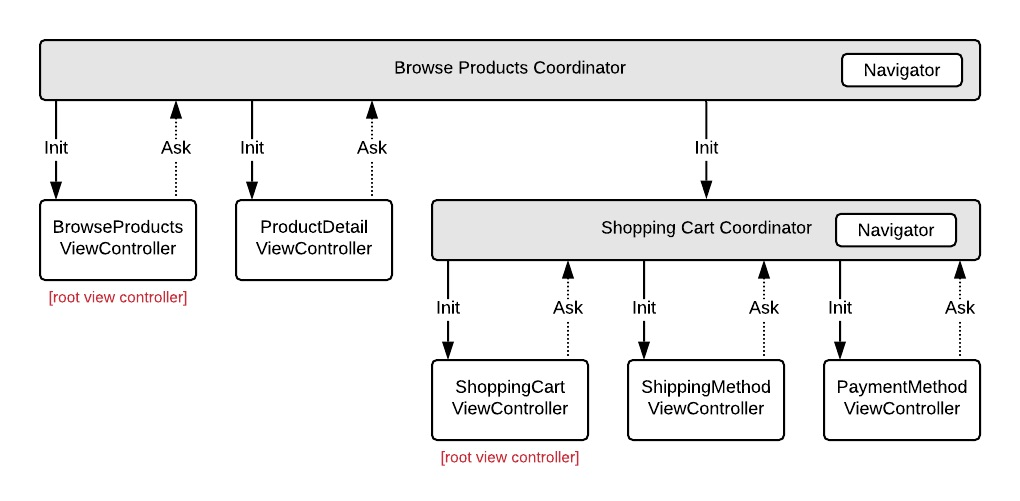
\includegraphics[width=10cm]{coordinator-example}
%     \captionof{figure}{
%        Esempio di coordinator pattern
%     }
%     \label{fig:5}
% \end{minipage}\\ \\

% Come si evince dall'immagine è presente in entrambi i coordinator è presente un oggetto
% \textbf{navigator} che sarà in gestore di un UINavigationController
\section{UIKit Dynamics}

Per la progettazione iniziale delle animazioni è stato fatto un attento studio a metodologie e frameworks
atti a creare animazioni interattive fluide.

Alla fine è stato deciso di utilizzare un pacchetto
nativo di iOS incluso nello UIKit\cite{uikit}, chiamato UIKit Dynamics\cite{uidynamics}: questo framework,
con una serie di API, offre delle funzioni di animazione base che 
donano alle viste i comportamenti fisici del mondo reale.

Il framework si basa su degli oggetti \textbf{UIDynamicAnimator} in cui ogni animator è responsabile delle
animazioni che avengono sulla sua \textbf{referenceView} e si inizializza 
attraverso la seguente funzione:

\begin{minted}{swift}
    UIDynamicAnimator.init(referenceView view: UIView)
\end{minted}

% una volta inizializzato attraverso la funzione addBehavior sarà posibile assegnargli
% dei comportamenti fisici predefiniti.

\subsection{Comportamenti base}

Ogni animator attraverso il metodo addBehavior puà assegnare a determinate
viste comportamenti fisici elencati sei seguito: 

\begin{itemize}
    % \item\textbf{UIDynamicBehavior}: il comportamento base da cui ereditano tutti gli altri;
    \item\textbf{UIAttachmentBehavior}: crea una relazione o legame tra due DynamicItem o tra un DynamicItem e un punto di ancoraggio;
    \item\textbf{UICollisionBehavior}: un oggetto che conferisce a un array di DynamicItems la possibilità di impegnarsi in collisioni tra loro e con i limiti specificati del comportamento
    \item\textbf{UIFieldBehavior}: un oggetto che conferisce delle proprietà magnetiche, elettriche a un DynamicItem;
    \item\textbf{UIGravityBehavior}: aggiunge all'oggeto un forza di gravità;
    \item\textbf{UIPushBehavior}: Aggiunge all'oggetto una forza continua o istantanea in una direzione specifica;
    \item\textbf{UISnapBehavior}: Un comportamento simile a una molla il cui movimento iniziale viene smorzato nel tempo in modo che l'oggetto si stabilizzi in un punto specifico.
\end{itemize}

Di seguito un esempio di implementazione degli strumenti UIDynamics in QIX

\begin{minipage}{\linewidth}
    \centering
    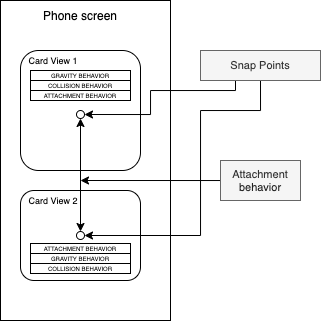
\includegraphics[width=10cm]{animation}
    \captionof{figure}{
       Schema dell'implementazione di UIDynamics
    }
    \label{fig:6}
\end{minipage}\\